\section{Results}
\label{sec:Results}


\subsection{Heidelberg University}

\begin{figure}[h!]
  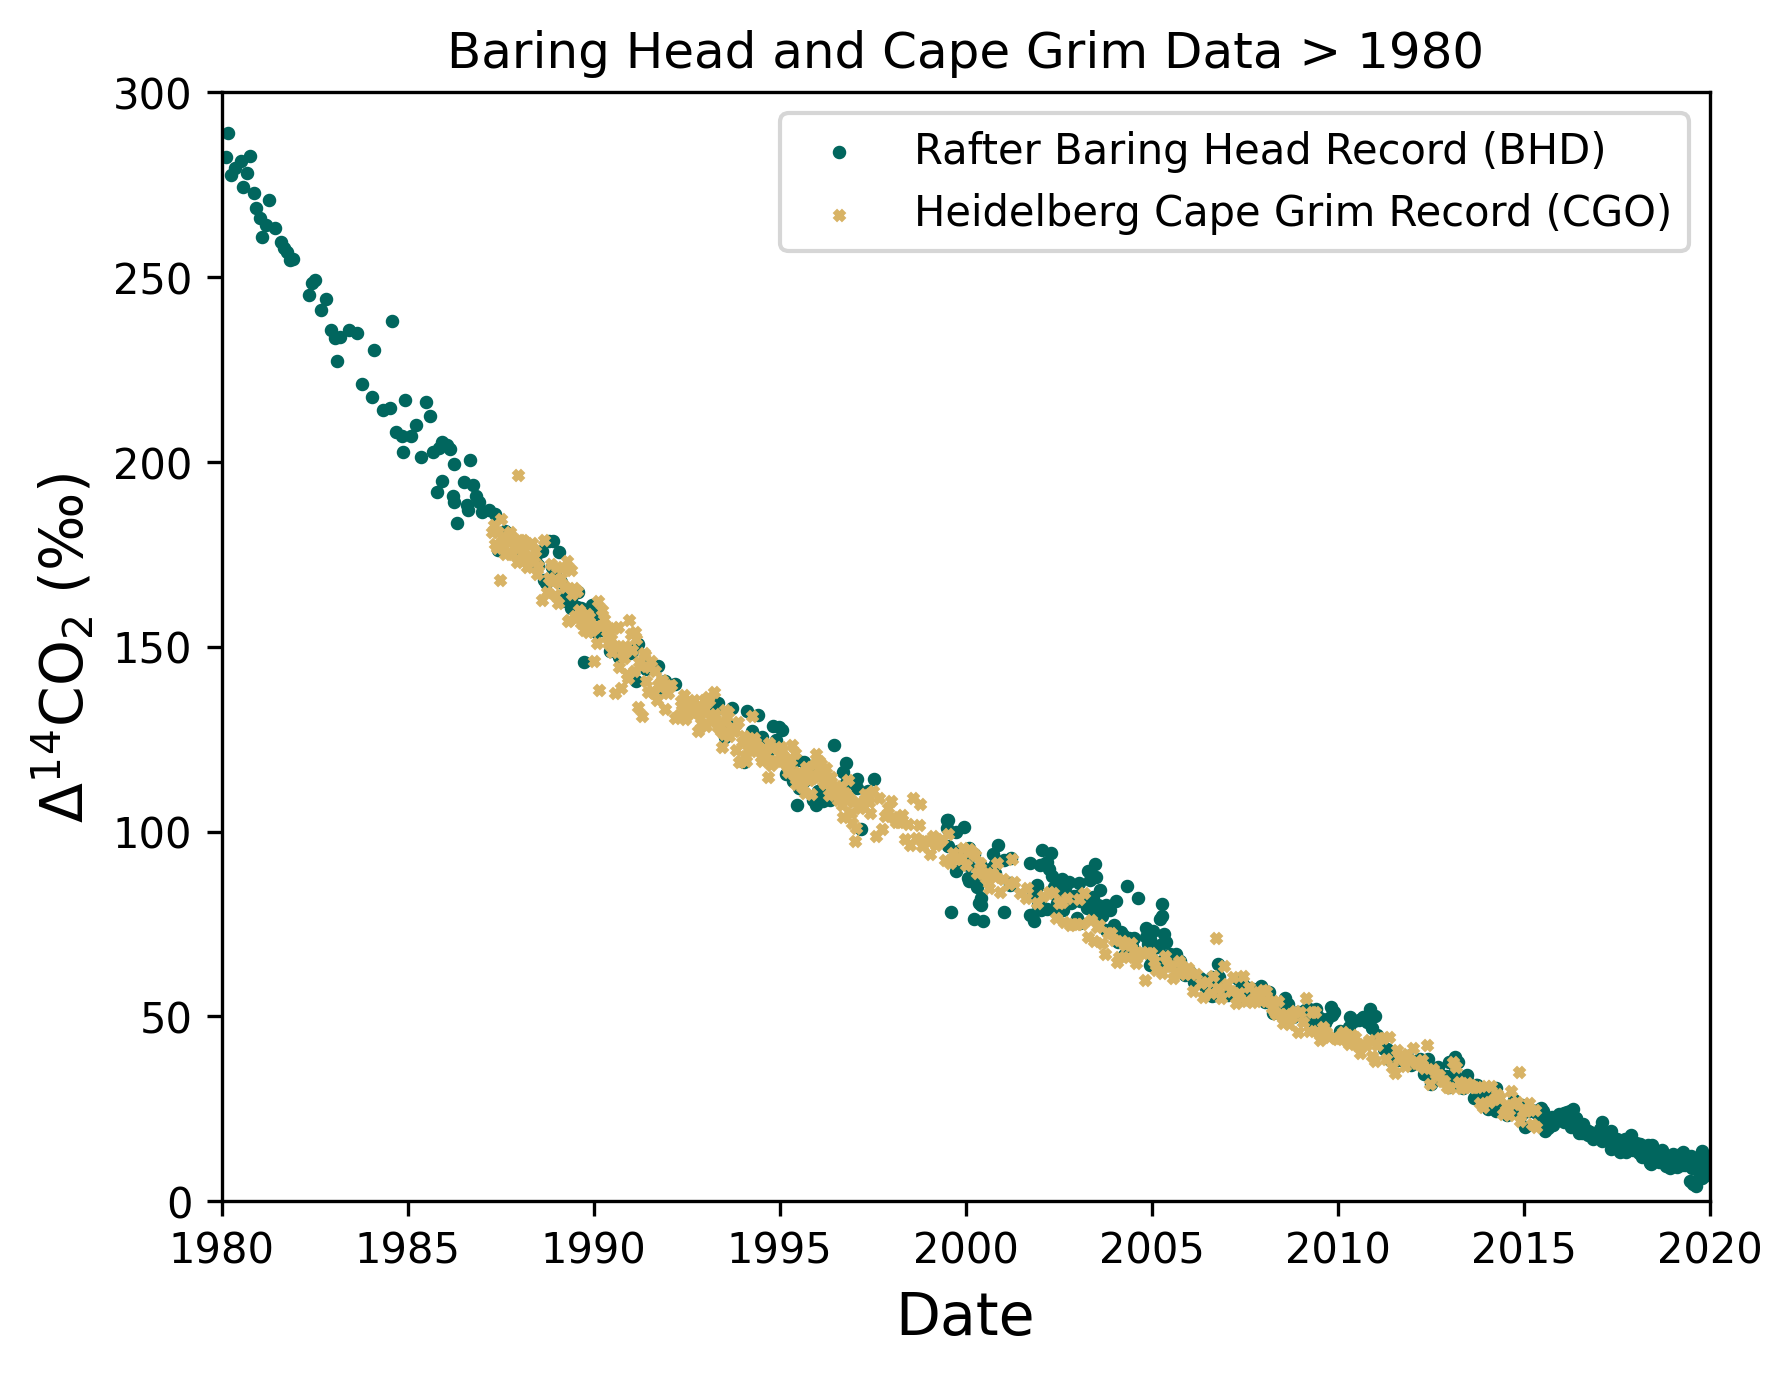
\includegraphics[width=1\textwidth]{/mnt/c/Users/clewis/IdeaProjects/GNS/Interlab_Comparison/output/DEV_FirstDraft_figure1.png}
  \caption{Visual summary of available data used for intercomparison between Heidelberg University and Rafter Radiocarbon Lab}
  \label{fig:results1}
\end{figure}


\begin{figure}[h!]
  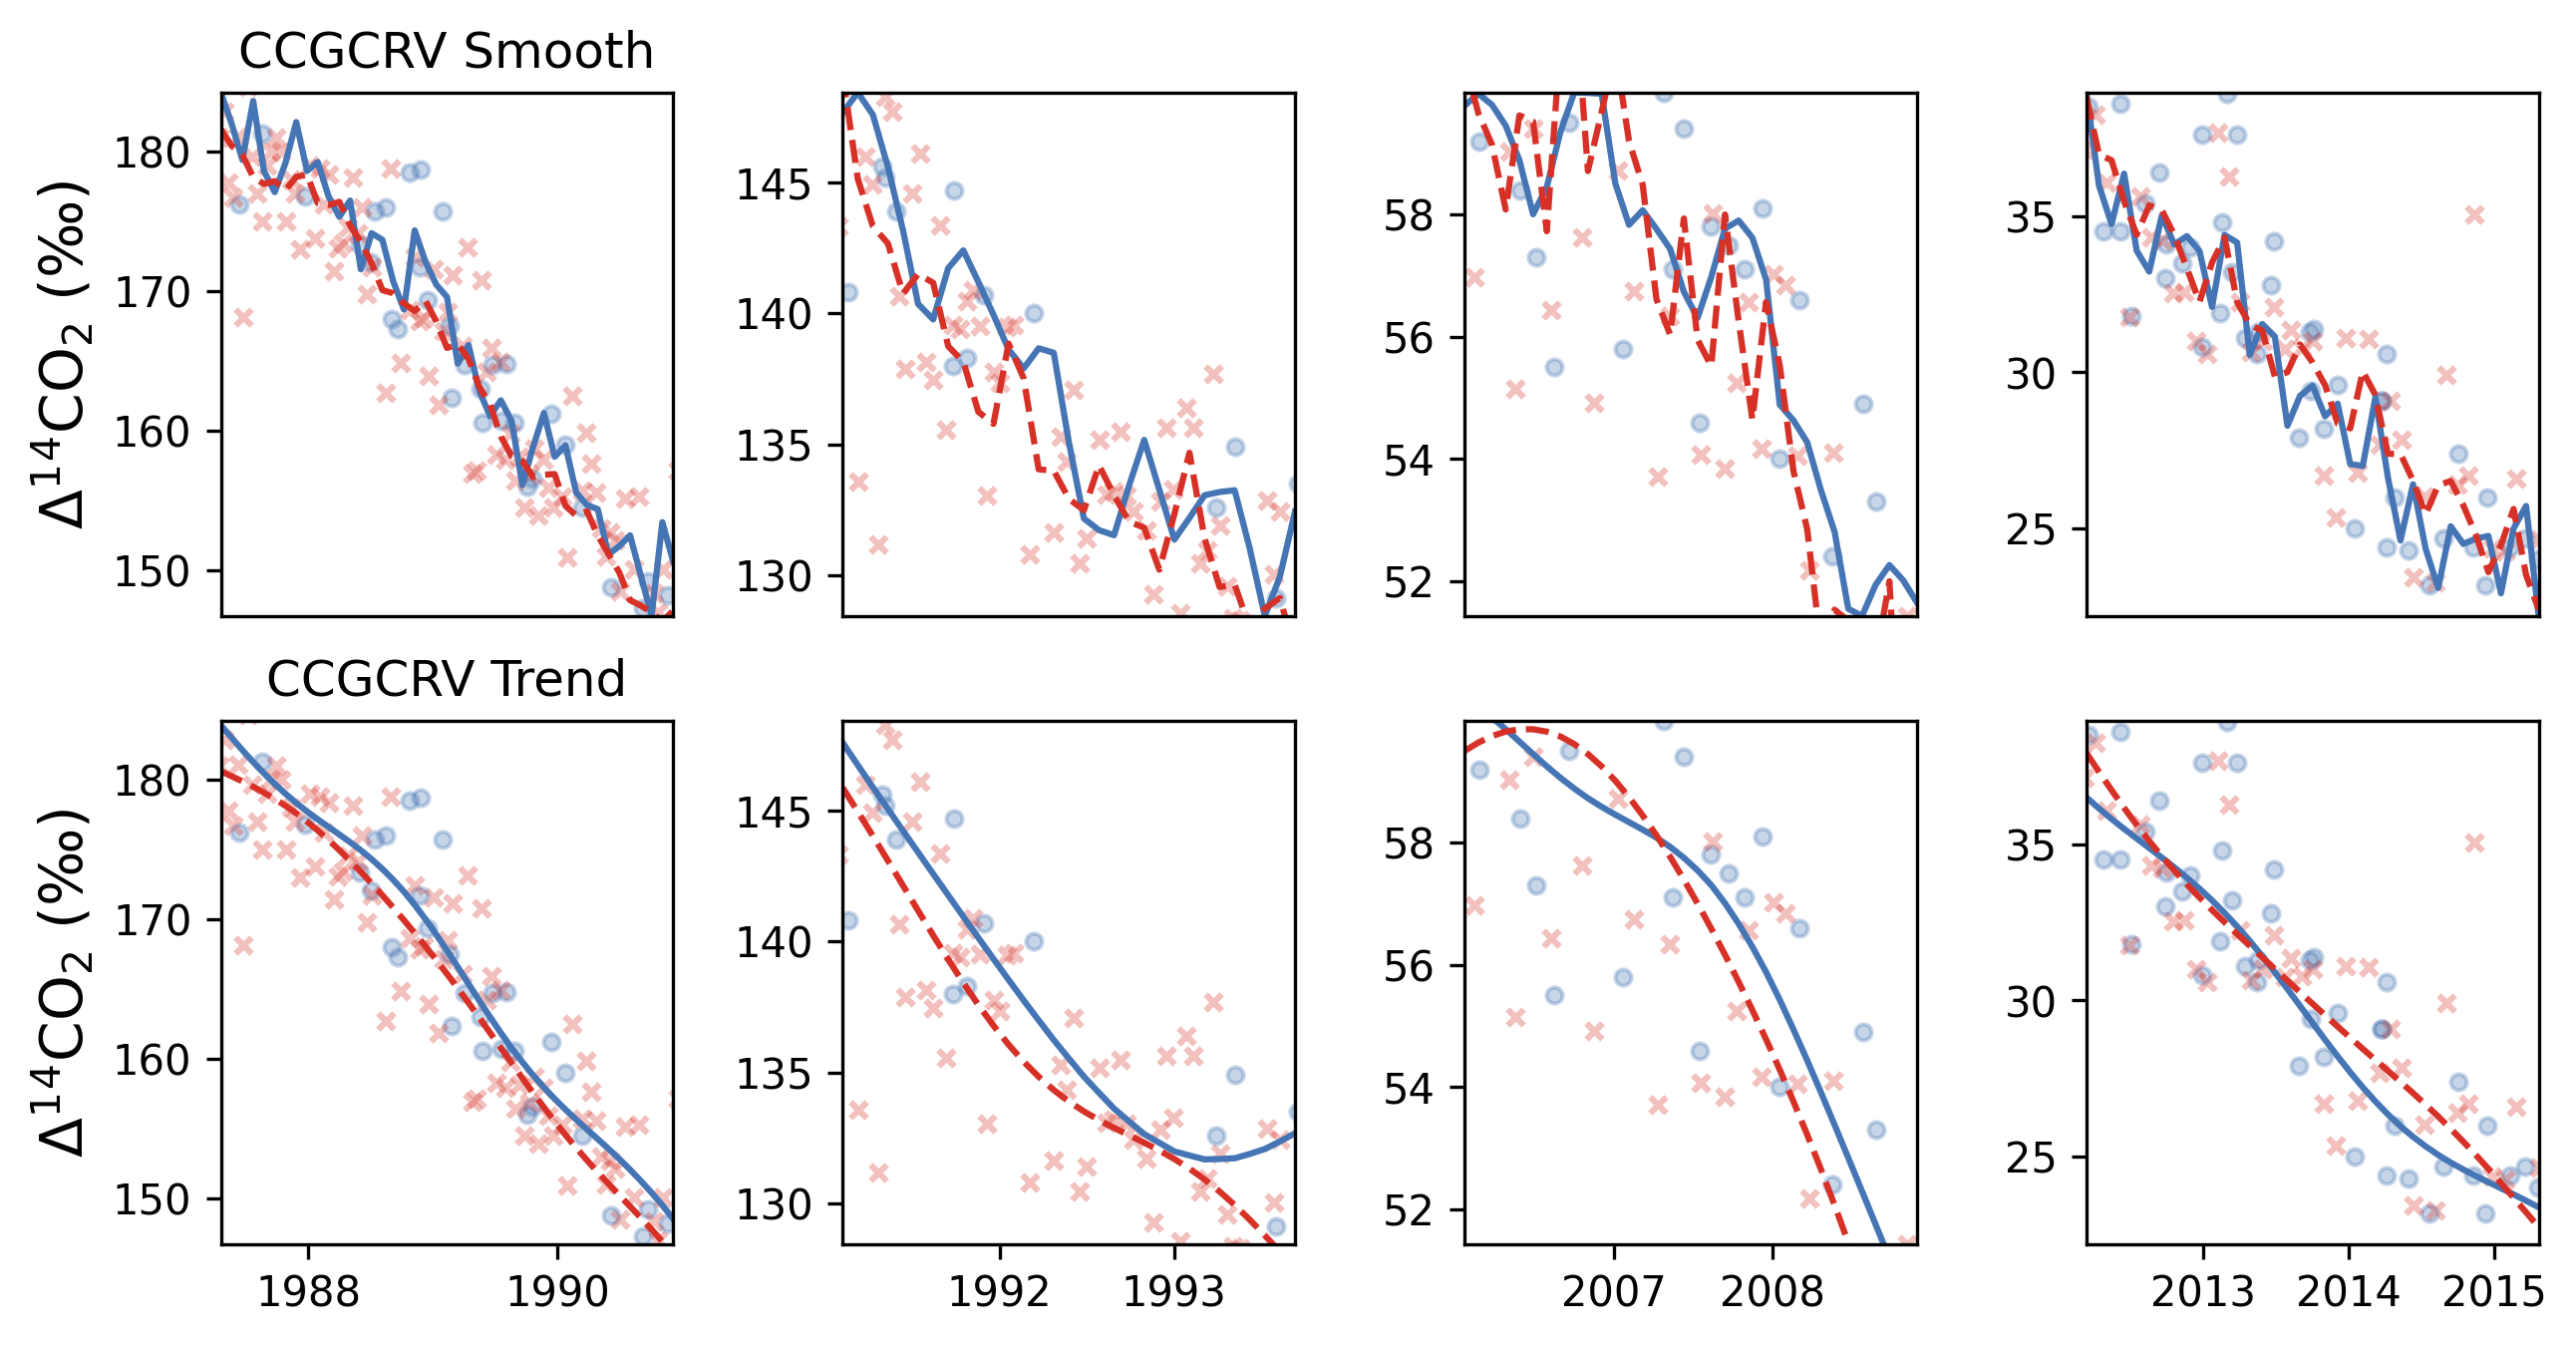
\includegraphics[width=1\textwidth]{/mnt/c/Users/clewis/IdeaProjects/GNS/Interlab_Comparison/output/DEV_FirstDraft_figure3b_D14C.png}
  \caption{Means of Monte Carlo simulation using CCGCRV "smooth" function (top panel), and "trend" function (bottom panel) overlaid upon initial CGO and BHD data. Panel a-d represents the various time-intervals used in this intercomparison: 1987 - 1991, 1991 - 1994, 2006 - 2009, 2012 - 2016}
  \label{fig:results1}
\end{figure}


\newpage
\subsection{ANSTO and University of Magallanes}
\begin{figure}[h!]
  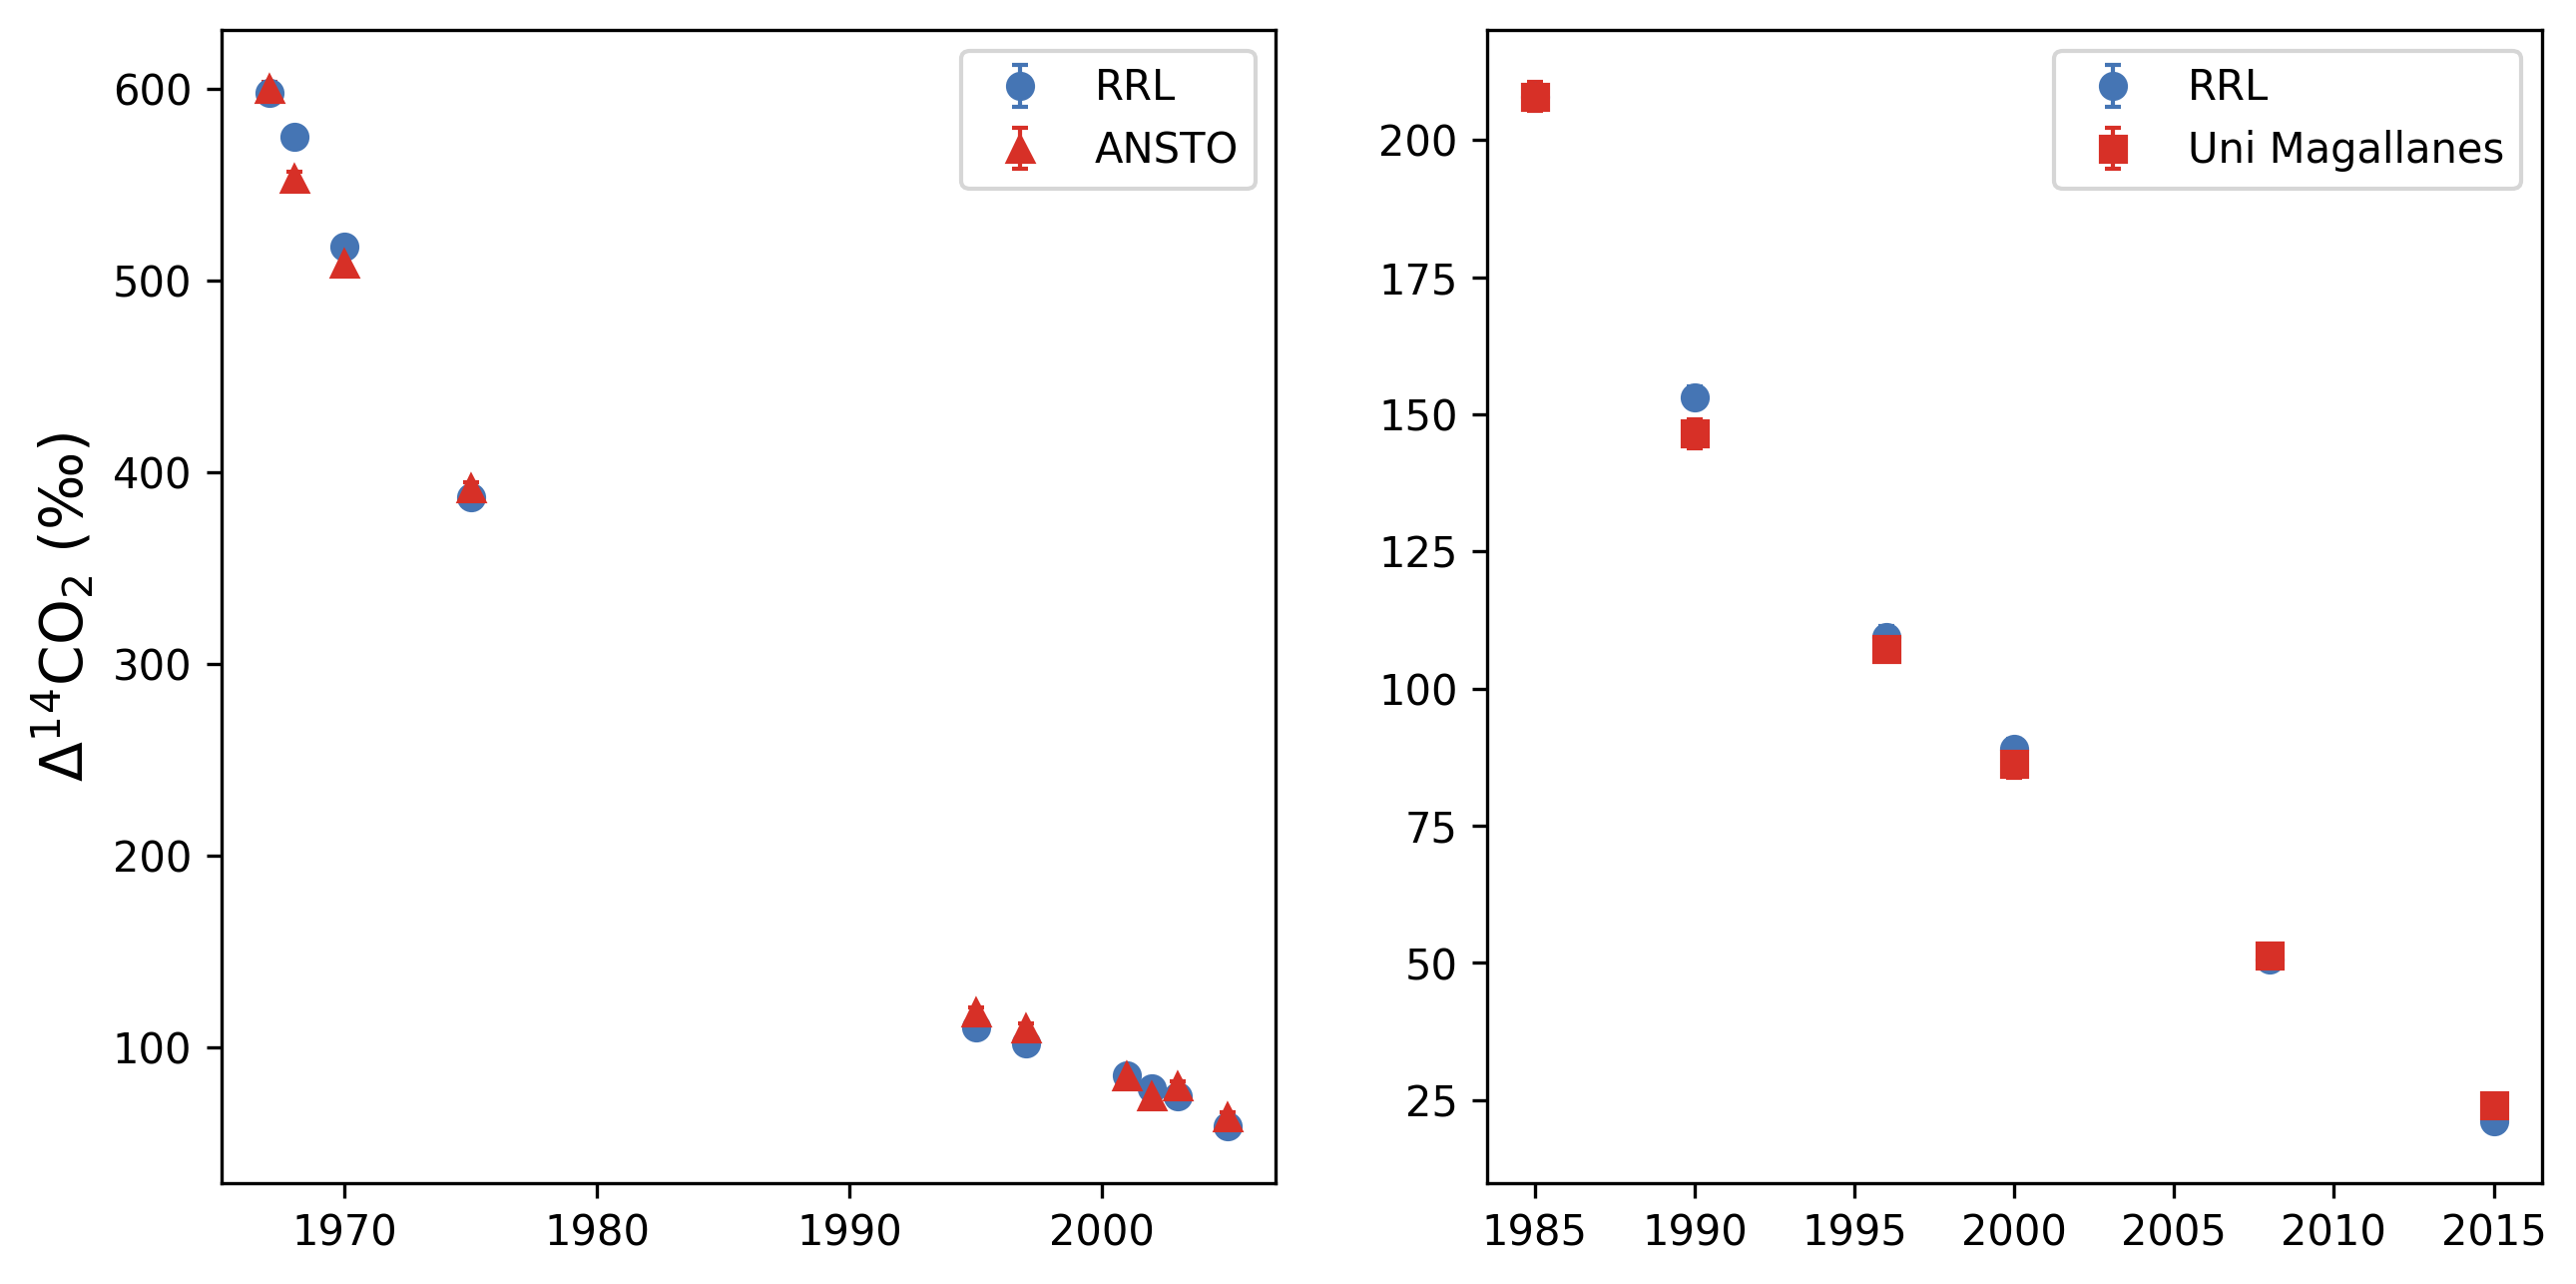
\includegraphics[width=1\textwidth]{/mnt/c/Users/clewis/IdeaProjects/GNS/Interlab_Comparison/output/Magallanes_Ansto_comb.png}
  \caption{ADD CAPTION LATER}
  \label{fig:results1}
\end{figure}

\newpage
\subsection{SIO / LLNL}

\begin{figure}[h!]
  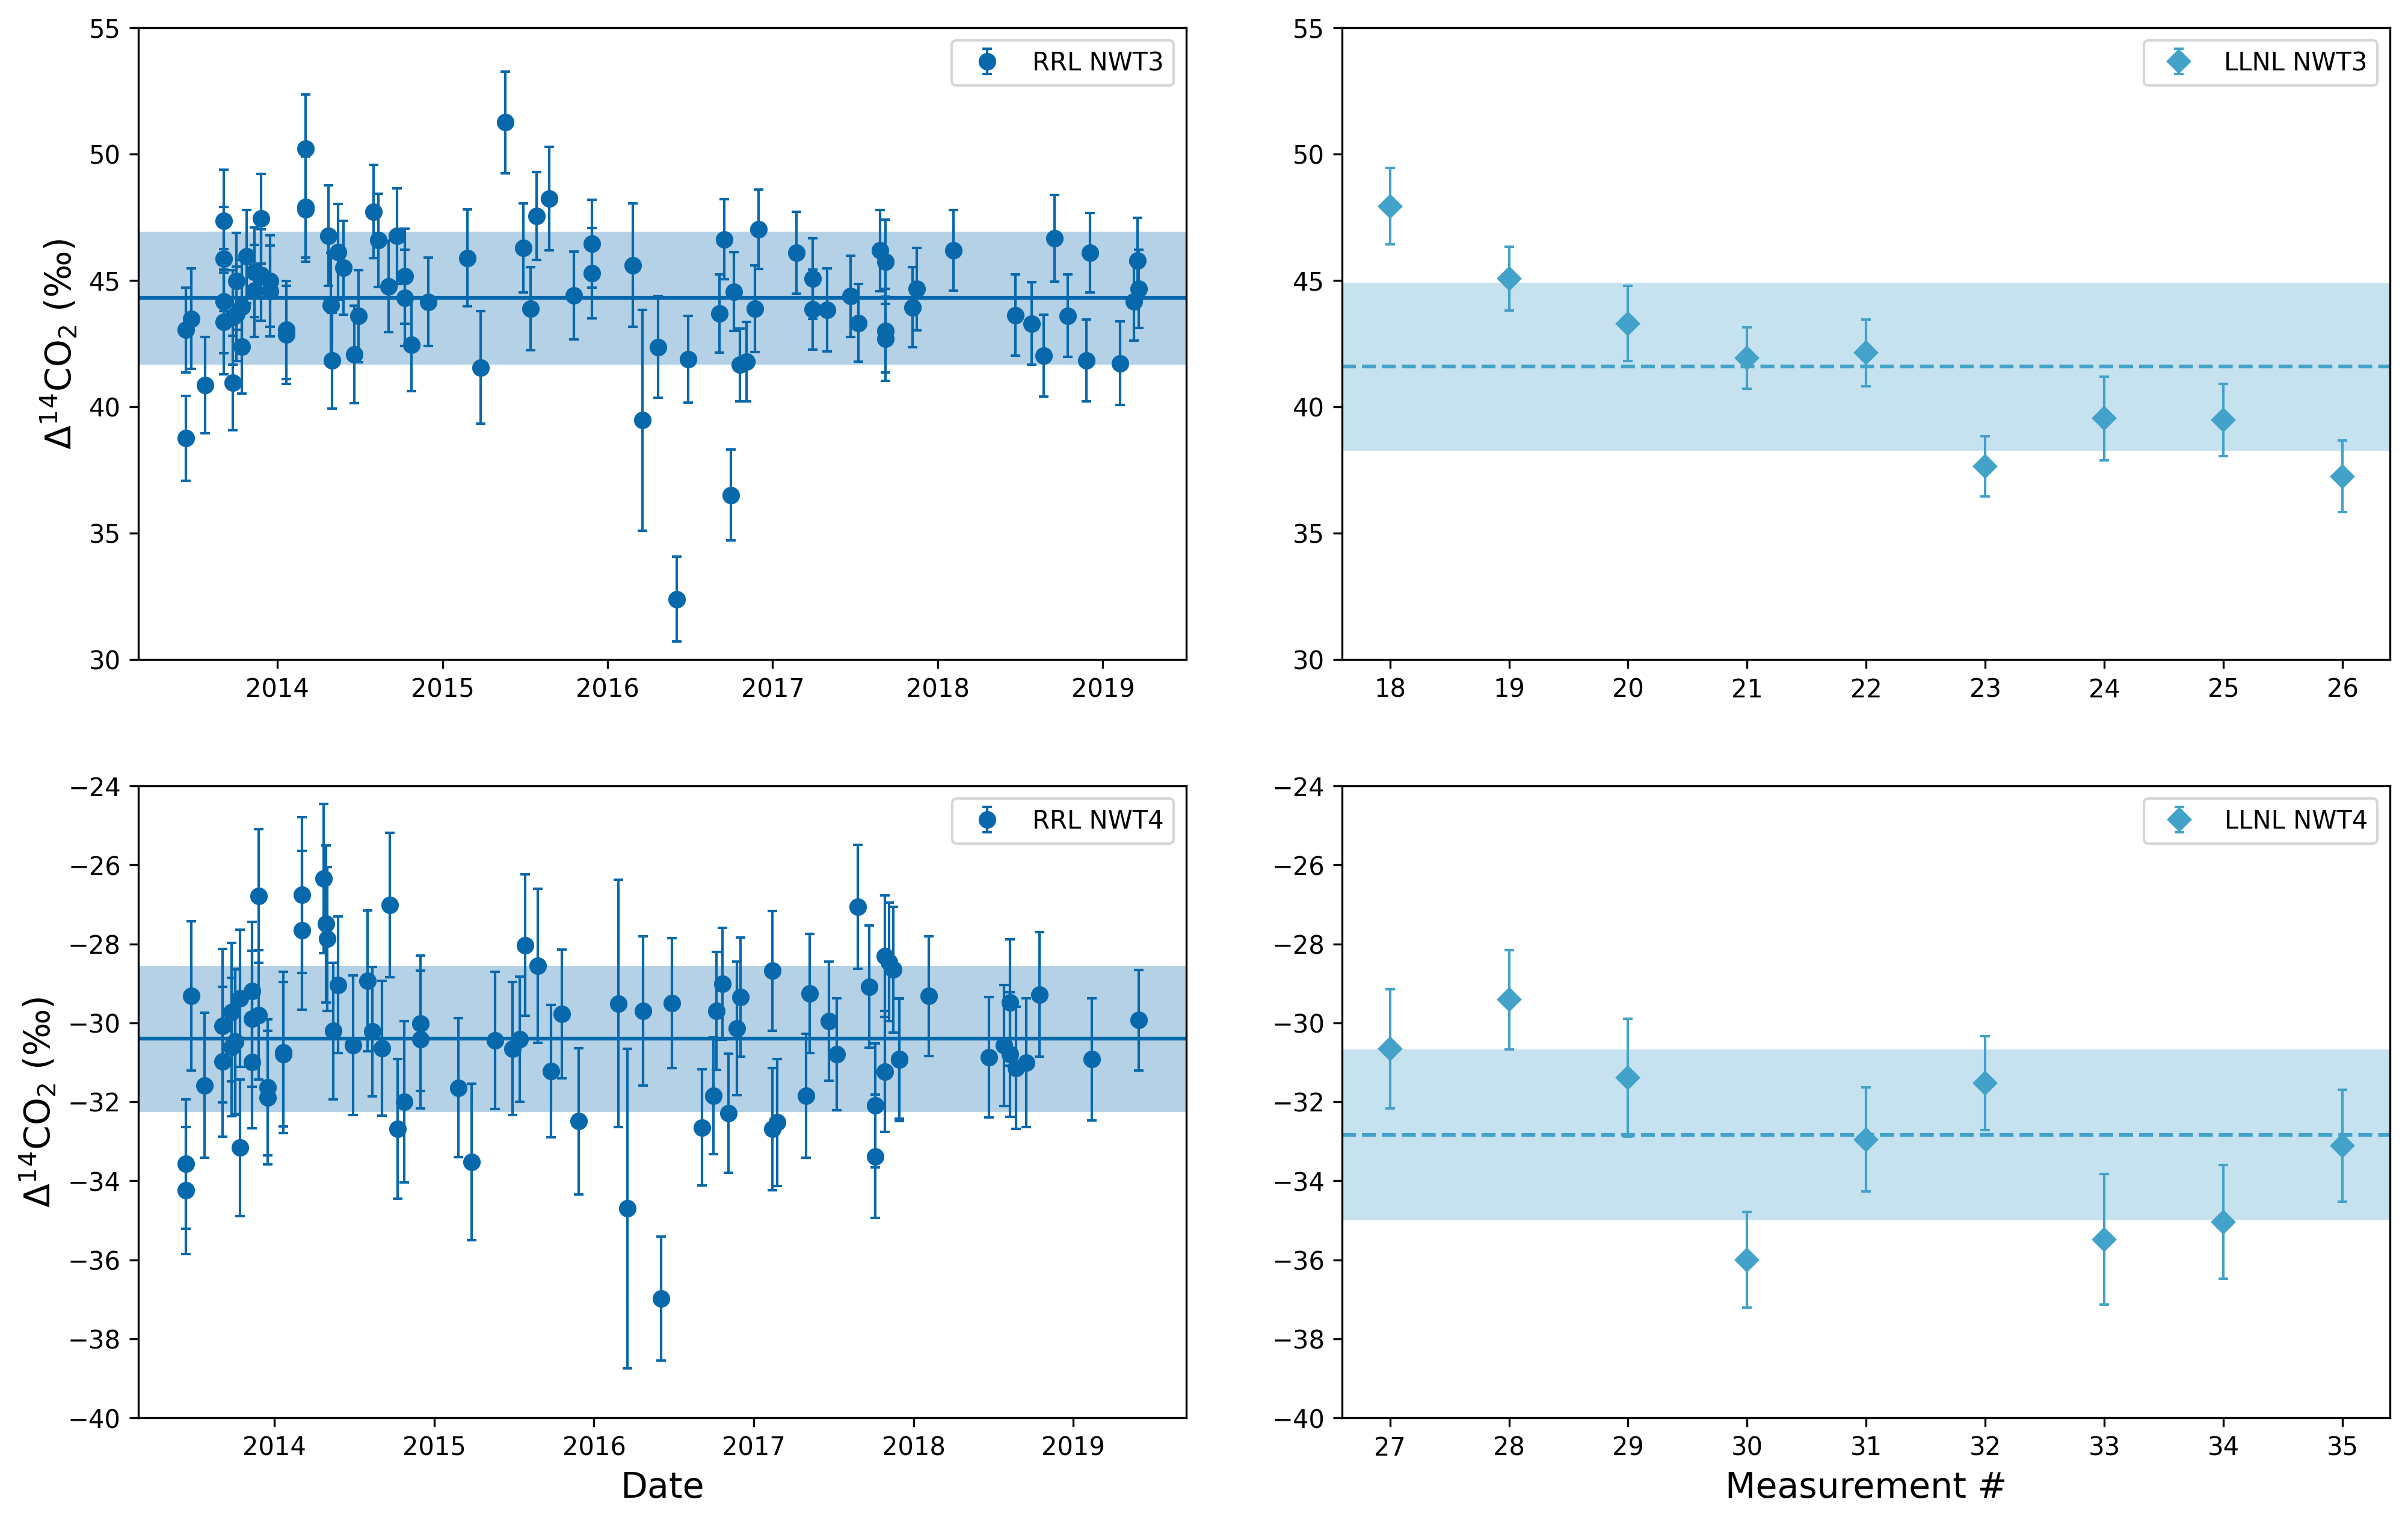
\includegraphics[width=1\textwidth]{/mnt/c/Users/clewis/IdeaProjects/GNS/Interlab_Comparison/output/SIOLLNLvRRL.png}
  \caption{Top panel shows ${\Delta^{14}CO_{2}}$ measurements of NWT3 standard from RRL (a) and SIO/LLNL (b), respectively. Bottom panel similarly shows NWT4 standard.}
  \label{fig:results1}
\end{figure}

\begin{tabular}{ |p{5cm}||p{2cm}|p{1.5cm}|p{3cm}|  }
 \hline
 \multicolumn{4}{|c|}{Result Summary } \\
 \hline
 Institute vs. RRL       &  ${\Delta\Delta^{14}C}$ &  p-value & Result\\
 \hline
Heidelberg [1987 - 1991] & 1.85\pm0.30 &  $3.0x10^{-7}$  & Different \\
Heidelberg [1987 - 1991] & 1.90\pm0.43  & $4.0x10^{-4}$ & Different  \\
Heidelberg [1987 - 1991] & 0.55\pm0.22  & 0.03 & Not different \\      
Heidelberg [1987 - 1991] & -0.52\pm0.26 & 0.02  & Not different  \\
SIO/LLNL(NWT3)          & 2.72\pm1.14 & 0.005   & Different  \\
SIO/LLNL(NWT4)           & 2.44\pm0.75 &  $4x10^{-4}$          & Different  \\
ANSTO                    & 0.46\pm2.76 & 0.878  & NOT different \\
 \hline
\end{tabular}







